%!TEX root = ../../Main.tex
\graphicspath{{Chapters/Project/}}
%-------------------------------------------------------------------------------

\section{Conclusion} % (fold)
\label{sec:conclusion}

% section conclusion (end)

Here is an inline equation $f(x) = ax+b$. 

\begin{figure}[H]
\centering
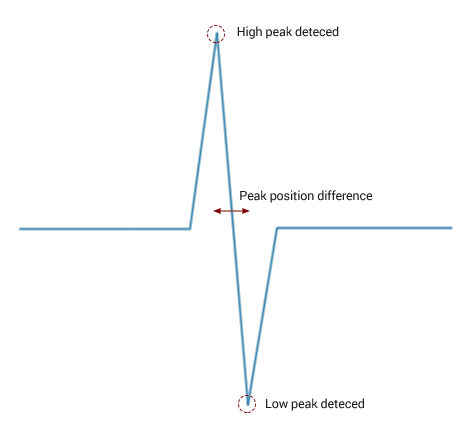
\includegraphics[width = 300 pt]{Img/Figures.png}
\caption{Block diagram}
\label{fig:BlockDiagram}
\end{figure}

\begin{equation}
\frac{n!}{k!(n-k)!} = \binom{n}{k}
\label{eq: myequation}
\end{equation}